\documentclass[../main.tex]{subfiles}
\begin{document}
% Babel (spanish) hace activos los caracteres < y >, lo que rompe la sintaxis
% de flechas de TikZ (->, >=Stealth). Los desactivamos como shorthand en esta unidad.
\shorthandoff{<>}
\section{Principios de Diseño de Seguridad y Vulnerabilidades}

\subsection{Introducción: qué son los principios de diseño}

Los \textbf{principios de diseño} son bases que promueven un diseño que tenga como resultado un sistema \textbf{robusto y seguro}. Son principios guía de \emph{alto nivel} que deben adaptarse a las necesidades puntuales de cada sistema, se basan en las recomendaciones de los modelos de seguridad y deben aplicarse en \textbf{todas las capas} en donde funciona el sistema (políticas/procesos, físico, red, computadora, aplicación, dispositivo). Son simples y restrictivos.

\begin{center}
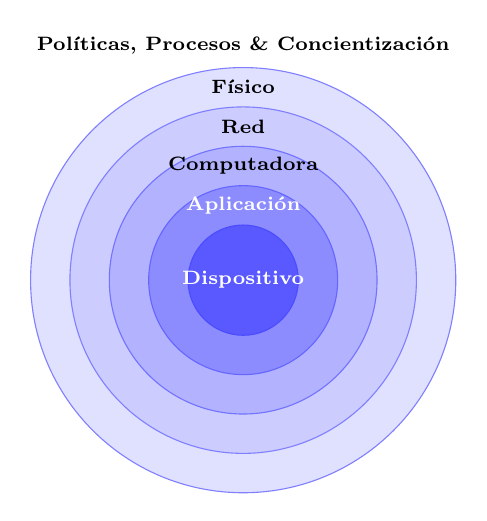
\begin{tikzpicture}
  % Capas concéntricas: del perímetro (externo) al dato (núcleo)
  \def\rA{2.7} \def\rB{2.2} \def\rC{1.7} \def\rD{1.2} \def\rE{0.7}
  \filldraw[fill=blue!12,draw=blue!50] (0,0) circle (\rA);
  \filldraw[fill=blue!20,draw=blue!50] (0,0) circle (\rB);
  \filldraw[fill=blue!30,draw=blue!55] (0,0) circle (\rC);
  \filldraw[fill=blue!45,draw=blue!60] (0,0) circle (\rD);
  \filldraw[fill=blue!65,draw=blue!70] (0,0) circle (\rE);
  \node[white] at (0,0) {\scriptsize\textbf{Dispositivo}};
  \node[white] at (0,{(\rD+\rE)/2}) {\scriptsize\textbf{Aplicación}};
  \node at (0,{(\rC+\rD)/2}) {\scriptsize\textbf{Computadora}};
  \node at (0,{(\rB+\rC)/2}) {\scriptsize\textbf{Red}};
  \node at (0,{(\rA+\rB)/2}) {\scriptsize\textbf{Físico}};
  \node at (0,{\rA+0.28}) {\scriptsize\textbf{Políticas, Procesos \& Concientización}};
\end{tikzpicture}
\end{center}
\diagcaption{Los principios se aplican en \emph{todas} las capas en las que vive el sistema, del perímetro (políticas/procesos) hacia el núcleo (el dato/dispositivo).}

\begin{destacado}
Que un sistema sea \textbf{robusto} significa que pueda aguantar cambios. El primer requisito de seguridad es que el sistema \textbf{esté disponible}: un ataque que tira el sistema (DoS) \emph{es} un ataque de seguridad, aunque no comprometa confidencialidad ni integridad.
\end{destacado}

Todo aspecto de seguridad involucra tres patas que conviven (no alcanza con sola la tecnología):
\begin{itemize}
  \item \textbf{Tecnología}: las herramientas (lo que más se ve en esta materia).
  \item \textbf{Procesos}: los procesos de las compañías; en sus grietas se mete la inseguridad.
  \item \textbf{Personas}: la pata psicológica / ingeniería social. \prof{Es el punto más crítico por donde el sistema cae.}
\end{itemize}

\begin{destacado}
La seguridad es un \textbf{balance entre tres cosas}: seguridad, funcionalidad y eficiencia/performance (``bueno, bonito y barato''). Un sistema muy seguro suele ser dificilísimo de usar. La seguridad siempre es tan fuerte como el \textbf{eslabón más débil} de la cadena.
\end{destacado}

\subsection{Principios de Saltzer \& Schroeder (1975)}

Propuestos en \textbf{1975} para el diseño de \emph{sistemas operativos seguros}. Demostraron aplicabilidad en diseños generales y sistemas modernos. Son la base de buenas prácticas modernas y estrategias de gobierno en todas las capas. Muchos vienen del escenario militar.

\begin{destacado}
El profe remarcó que estos principios ``hay que grabarlos afuera porque son los más importantes''. Aparecen todo el tiempo de una u otra manera y \textbf{están todos conectados / se tocan entre sí}. El objetivo de la materia es generar la \textbf{intuición} para aplicarlos.
\end{destacado}

\subsubsection{1. Mínimo privilegio (Least privilege)}
Se debe asegurar que los sujetos (personas, entidades, procesos) sólo tengan el \textbf{acceso necesario} (la menor cantidad de permisos/capacidades) para realizar su trabajo, y nada más.
\begin{itemize}
  \item Ejemplo: en un sistema con información financiera confidencial, limitar quién accede. La persona que atiende el teléfono no necesita acceder a todo; el administrador de cuentas sí, pero \emph{no} a las cuentas que no administra.
  \item Por detrás surge que la \textbf{condición por default es no tener acceso a nada}.
\end{itemize}

\begin{definicion}{Mínimo privilegio}
Dar a cada sujeto únicamente los permisos/capacidades mínimas necesarias para realizar la tarea que tiene que hacer, y ningún permiso adicional. Por default no se tiene acceso a nada.
\end{definicion}

\subsubsection{2. Fallar de forma segura (Fail-safe defaults)}
Conectado al anterior: el default es ``no dejo entrar a nadie''.
\begin{itemize}
  \item A la hora de revisar, las \textbf{listas de permitidos (whitelists)} son mejores que las listas de excluidos (\textbf{blacklists}). Conviene marcar quién \emph{puede} entrar, no quién no puede. (Ejemplo del profe: Twitter pasó de white-listing a black-listing por razones económicas/de influencia, pero en general el white-listing es mejor.)
  \item Un sistema no abre puertos innecesariamente; por default los firewalls están encendidos.
  \item No hay cuentas de usuario por defecto con contraseña conocida.
  \item Un sistema que presenta una falla en un proceso o control de seguridad debe moverse a un \textbf{estado seguro}.
  \item Ejemplo: si el sistema de autenticación no puede conectarse a la base de datos para verificar un password, debe \textbf{rechazar el pedido} y no asignar permisos, por más que sean los mínimos. Lo que se penaliza al fallar seguro es \emph{funcionalidad}.
\end{itemize}
Ejemplo extremo de hardware: las normas FIPS de dispositivos físicos (HSM, criptochips/tokens) tienen niveles (1 a 4); en nivel 4, ante una amenaza física el dispositivo debe desaparecer o no debe haber forma de extraer la clave privada (anti-tampering).

\subsubsection{3. Simplicidad (Economy of mechanism)}
La complejidad es enemiga de la seguridad. Se debe evitar arquitecturas muy sofisticadas al desarrollar controles de seguridad.
\begin{itemize}
  \item Las soluciones complejas \textbf{exponen más superficie de ataque}, son menos robustas y más difíciles de entender; es más fácil que se cuelen bugs que deriven en vulnerabilidades explotables.
  \item Busca reducir la superficie de ataque y la complejidad de datos: p.\,ej. reducir al mínimo la cantidad de tuplas \textbf{(sujeto, acceso, objeto)}. Cada acceso es susceptible de ser explotado.
\end{itemize}

\subsubsection{4. Mediación completa (Complete mediation)}
Si hay un control, este debe aplicar a \textbf{todas} las interacciones alcanzadas.
\begin{itemize}
  \item Es ``la puerta del castillo'': todo pasa por ahí y no hay ningún otro mecanismo posible.
  \item El muestreo de algunas transacciones, controles al azar o entidades por fuera del control son problemas potenciales. No tiene sentido construir un muro y dejar la puerta abierta por el costado.
\end{itemize}

\subsubsection{5. Sistema/Diseño abierto (Open design)}
No debe basarse la seguridad en mantener el diseño oculto (no ``seguridad por oscuridad/ofuscación'').
\begin{itemize}
  \item Es el principio de Kerckhoffs aplicado: en encripción lo que se guarda es la \textbf{clave} (y se cambia frecuentemente); el \textbf{algoritmo es público} y conocido por todos. El mismo concepto aplica a los controles de seguridad.
  \item Todo secreto conocido por al menos una persona puede ser revelado. \prof{Los bits son eternos.} (Asumir que todo lo digitalizado puede llegar a verse / perderse.)
  \item Matiz: que NO deba basarse en ofuscación \textbf{no significa} que tenga que ser abierto y que todos se enteren. La ofuscación da algo de complejidad y tiempo (por eso los algoritmos militares son ocultos, aunque sigan también este principio); sirve como \emph{capa adicional}, no como única defensa.
  \item Pata de software libre/open source: es bueno porque tiene más \textbf{escrutinio} (más ojos $\Rightarrow$ menos bugs explotables). Hoy hay que tomarlo con pinzas: si bots meten commits automáticos en open source, el principio se rompe (importa que haya un \textbf{responsable} que responda).
\end{itemize}

\subsubsection{6. Separación / Segregación de privilegios (Separation of privilege)}
Toda tarea crítica no debe quedar bajo el control de un solo sujeto; más de un sujeto debe ser parte del proceso para asegurar un control entre partes.
\begin{itemize}
  \item Se aplica el principio de \textbf{control por oposición de intereses}: las partes tienen objetivos opuestos y en el equilibrio se evita el abuso.
  \item Ejemplo (ventas): para aprobar una venta con descuento, el vendedor (que quiere descontar mucho para cerrar) pide aprobación al financiero (que quiere descontar lo menos posible). Hay oposición de intereses.
  \item En seguridad informática: que no sea el mismo quien controla las claves de la base de datos y quien controla el sistema de pagos; si controlara la base, podría crearse un usuario con permisos para operar el sistema de pagos (``salto'').
  \item Puede contradecir el principio de simplicidad (agrega complejidad): ahí está el balance.
\end{itemize}

\begin{examen}
\textbf{Vínculo no trivial (clave para el parcial):} el profe relaciona ``\textbf{separar las credenciales del sistema de las del usuario}'' con el principio de \textbf{separación de privilegios}. Otro vínculo: mediación completa (única) + separación de privilegios $\Rightarrow$ la mediación de seguridad es única, pero el \emph{privilegio de controlarla} se separa para que no haya un único punto de falla.
\end{examen}

\subsubsection{7. Mecanismos exclusivos (Defense-in-Depth)}
Tiene dos partes:
\begin{itemize}
  \item \textbf{Exclusividad}: evitar que distintos mecanismos compartan recursos, algoritmos y hardware. Si algo es para seguridad, debe ser un mecanismo \textbf{exclusivo} para eso y nada más.
  \item \textbf{Defensa en profundidad}: diseñar controles compensatorios / de mitigación / reacción que se accionen si otro control falla o es superado.
\end{itemize}
Ejemplo (fuente de bugs/vulnerabilidades): un \textbf{flag} que originalmente indica ``el cliente puede comprar'' se reutiliza después también para ``puede recibir un voucher'' (asunción \emph{as-is}/correlación que se mantendría eterna). Cuando esa correlación se rompe, el código queda mezclado: un mismo flag significa dos cosas. Si alguien controla indirectamente ese parámetro, rompe la exclusividad y puede saltar de un sistema a otro (relacionado con \emph{pivoting}). Ejemplo análogo físico: una llave/flag de acceso a una puerta importante a la que implícitamente se ató el acceso a un servidor; el personal de limpieza con esa llave queda con acceso al servidor.

\begin{examen}
\textbf{Defensa en profundidad} (remarcado en la clase de consulta): encadenar controles para \textbf{maximizar cuántas cosas hay que romper} para vulnerar el sistema. Ejemplo del PDF: se hace segregación de tareas + mínimos privilegios, pero una vulnerabilidad permite llevar adelante una venta sin autorizaciones $\Rightarrow$ ¿qué controles se agregan para monitorearla? ¿alertas que bloqueen la transacción? ¿una confirmación?
\end{examen}

\begin{center}
\begin{tikzpicture}[
    ctrl/.style={draw=blue!60,fill=blue!12,rounded corners=2pt,
                 minimum width=5.2cm,minimum height=0.62cm,font=\footnotesize}]
  \node[ctrl] (c1) {Mínimo privilegio};
  \node[ctrl,below=2pt of c1] (c2) {Segregación de tareas};
  \node[ctrl,below=2pt of c2] (c3) {Mediación completa};
  \node[ctrl,below=2pt of c3] (c4) {Monitoreo / alertas que bloquean};
  \node[ctrl,below=2pt of c4] (c5) {Confirmación / compensación};
  \node[draw=red!70,fill=red!12,rounded corners=2pt,minimum width=5.2cm,
        minimum height=0.55cm,font=\footnotesize\bfseries,below=4pt of c5] (act) {ACTIVO a proteger};
  % El atacante debe romper TODAS las capas
  \draw[->,red!70,thick] (-3.6,0.3) node[left,font=\scriptsize,red!70]{atacante} -- (-3.0,0.3);
  \draw[decorate,decoration={brace,amplitude=5pt},blue!60]
        (3.1,0.45) -- (3.1,{-0.62*5 -2pt*5 -0.4}) node[midway,right=4pt,font=\scriptsize,align=left]{hay que\\ romper\\ \emph{todas}};
\end{tikzpicture}
\end{center}
\diagcaption{Defensa en profundidad: se \textbf{encadenan} controles independientes. Si uno falla o es superado, otro lo compensa; el atacante debe vulnerar todas las capas para llegar al activo.}

\subsubsection{8. Menor asombro / Aceptación psicológica (Psychological acceptability)}
\begin{itemize}
  \item El \textbf{peor enemigo} de cualquier diseño de seguridad es el \textbf{usuario no alineado}; el mejor aliado es el usuario comprometido con la seguridad.
  \item Los controles deben ser simples de usar, incluso para alguien sin conocimientos técnicos, y no deben complicar el negocio ni sus procesos.
  \item La \textbf{concientización} del problema y del valor de la seguridad es fundamental para lograr la aceptación del control.
\end{itemize}

\begin{destacado}
\prof{Los muy buenos trabajadores son malos usuarios de seguridad.} Los más eficientes saben ``navegar la burocracia'' y van a saltear las restricciones de seguridad para resolver el problema. Por eso hay que capacitarlos para que entiendan que mantener la seguridad es parte de su trabajo. Un buen esquema asume que la persona \emph{va a} intentar saltarlo y diseña para que eso sea una excepcionalidad controlada y consciente. Caso real: un compañero pasó dos meses mejorando la seguridad de la página rastreadora de ambulancias, y luego el jefe de ambulancias consiguió por ``rosca'' el mismo usuario con todos los permisos porque el negocio lo requería.
\end{destacado}

\begin{ojo}
La seguridad ``no tiene límite'' (es un \emph{bounder}): se puede poner tanta como la paranoia diga. El sistema más seguro del universo sería imposible de usar. Hay que balancear con experiencia de usuario (UX), pensando las cosas centradas en las personas.
\end{ojo}

\subsection{La seguridad NO se garantiza}

\begin{ojo}
\textbf{GANCHO/TRAMPA que penaliza.} \prof{Garantizar la seguridad es algo que no se puede hacer jamás.} Ante la pregunta ``¿me garantizás que esto es seguro?'', nadie idóneo dice ``sí, te lo garantizo'': es muy caro, requiere conocimiento muy específico y aún así es muy difícil por todo lo que ocurre \emph{fuera} del sistema (el ecosistema de infraestructura/redes donde funciona).

\textbf{Construir software de CALIDAD NO es garantía de seguridad} (V/F $\Rightarrow$ \textbf{FALSO} la afirmación ``calidad = seguro''; Recup 2025). Afirmar que algo ``garantiza la seguridad'' o que ``software de calidad = seguro'' \textbf{penaliza}.
\end{ojo}

Por eso, saliendo de los mecanismos específicos, la seguridad se trata como un problema de \textbf{gestión de riesgo}. Amenaza y vulnerabilidad componen dos probabilidades. Frente a un riesgo se puede:
\begin{itemize}
  \item \textbf{Eliminarlo}.
  \item \textbf{Mitigarlo} (reducir la probabilidad o el impacto; p.\,ej. backups en otra nube).
  \item \textbf{Compensarlo} (no se evita, pero se agrega p.\,ej. una alerta que avisa cuando pasa).
  \item \textbf{Aceptarlo} (documentarlo y no hacer nada): a veces es la solución más efectiva cuando evitarlo es carísimo (en dinero o en UX). Lo importante es que la decisión se tome con conciencia.
\end{itemize}

\subsection{Calidad/Procesos: DevOps vs DevSecOps vs MLOps}

\begin{examen}
\textbf{``Seguridad de la Información'' NO es un componente de DevOps} --- pertenece a \textbf{DevSecOps} (el agregado de \emph{Sec}). Hoy además se suma \textbf{MLOps} (operaciones de machine learning). Errores que penalizan: ubicar la seguridad como parte nativa de DevOps.
\end{examen}

\subsection{Modelado de amenazas (Threat Modeling)}

Es una técnica de ingeniería para entender las \textbf{amenazas, ataques, vulnerabilidades y contramedidas} que pueden afectar a una aplicación. Define la tarea de modelar las amenazas al negocio en la \textbf{superficie de ataque}; con el modelo y la clasificación de amenazas se definen contramedidas específicas. Debe incluir inteligencia, tendencias y ataques pasados, y es un \textbf{proceso continuo} (las amenazas cambian). Se usa para mejorar el diseño y reducir el riesgo.

\textbf{Proceso (Microsoft / OWASP, similares):}
\begin{enumerate}
  \item Definir el alcance (acotar el esfuerzo para que cubra lo suficiente sin excederse).
  \item Determinar / definir amenazas (diagramar dependencias, identificar caminos de explotación).
  \item Definir contramedidas y mitigación.
  \item Revisar el trabajo, los cambios y volver a empezar (validar).
\end{enumerate}

\subsubsection{Modelo STRIDE}

\begin{examen}
STRIDE \textbf{es de Microsoft} (V/F, 2015 $\Rightarrow$ Verdadero: ``fue desarrollado por Microsoft''). Es conocimiento \textbf{``enciclopédico'' exigible}: hay que saber de memoria qué significa cada letra y qué propiedad viola. Surge en la época de Windows 98 cuando se cuestionaba mucho la seguridad de Windows.
\end{examen}

Clasifica las amenazas en \textbf{6 categorías}. La idea del modelo: por cada sistema, conseguir al menos 2 amenazas críticas en cada categoría.

\begin{center}
\begin{tabular}{|c|l|l|l|}
\hline
 & \textbf{Amenaza} & \textbf{Propiedad violada} & \textbf{Definición} \\
\hline
\textbf{S} & Spoofing & Autenticación & Hacerse pasar por algo/alguien que no se es \\
\hline
\textbf{T} & Tampering & Integridad & Modificar algo en disco, red, memoria, etc. \\
\hline
\textbf{R} & Repudiation & No repudio & Negar haber hecho algo (sin poder probarlo) \\
\hline
\textbf{I} & Information Disclosure & Confidencialidad & Revelar información a quien no debe acceder \\
\hline
\textbf{D} & Denial of Service & Disponibilidad & Agotar recursos necesarios para dar el servicio \\
\hline
\textbf{E} & Elevation of Privilege & Autorización & Permitir hacer algo para lo que no se está autorizado \\
\hline
\end{tabular}
\end{center}

\begin{center}
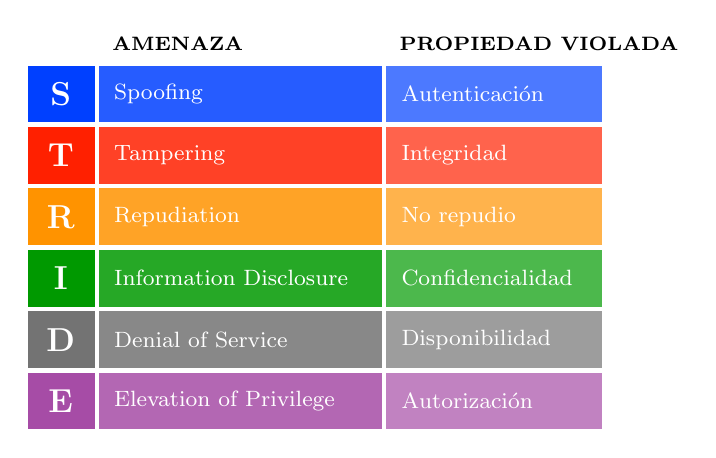
\begin{tikzpicture}[
    letter/.style={minimum width=0.7cm,minimum height=0.72cm,font=\bfseries\large,
                   text=white,anchor=center},
    cell/.style={minimum height=0.72cm,font=\footnotesize,anchor=west,text=white,
                 inner sep=4pt},
    row/.style={draw=white,line width=1.2pt}]
  \def\h{0.78}
  % colores por categoría (estilo slide), como nombres simples para poder mezclarlos
  \colorlet{colS}{blue!75!cyan}
  \colorlet{colT}{red!75!orange}
  \colorlet{colR}{orange!85!yellow}
  \colorlet{colI}{green!60!black}
  \colorlet{colD}{black!55}
  \colorlet{colE}{violet!70}
  \foreach \i/\L/\col/\amen/\prop in {
      0/S/colS/Spoofing/{Autenticación},
      1/T/colT/Tampering/{Integridad},
      2/R/colR/Repudiation/{No repudio},
      3/I/colI/Information Disclosure/{Confidencialidad},
      4/D/colD/Denial of Service/{Disponibilidad},
      5/E/colE/Elevation of Privilege/{Autorización}}{
    \fill[\col] (0,-\i*\h) rectangle (0.85,-\i*\h-0.72);
    \fill[\col!85] (0.9,-\i*\h) rectangle (4.5,-\i*\h-0.72);
    \fill[\col!70] (4.55,-\i*\h) rectangle (7.3,-\i*\h-0.72);
    \node[letter] at (0.42,-\i*\h-0.36) {\L};
    \node[cell] at (0.95,-\i*\h-0.36) {\amen};
    \node[cell] at (4.6,-\i*\h-0.36) {\prop};
  }
  \node[font=\scriptsize\bfseries] at (0.42,0.28) {};
  \node[font=\scriptsize\bfseries,anchor=west] at (0.95,0.28) {AMENAZA};
  \node[font=\scriptsize\bfseries,anchor=west] at (4.6,0.28) {PROPIEDAD VIOLADA};
\end{tikzpicture}
\end{center}
\diagcaption{Las 6 categorías STRIDE y la propiedad de seguridad que viola cada una (memorizar: cada letra $\leftrightarrow$ su propiedad).}

\subsubsection{DFD (Data Flow Model) + STRIDE}
El DFD representa las partes de un sistema y los riesgos de cada una. Analiza elementos de cada categoría:
\begin{itemize}
  \item \textbf{Procesos}: contenedores, procesos ejecutables.
  \item \textbf{Entidades externas} al sistema: personas, otros sistemas.
  \item \textbf{Flujos de datos}: comunicaciones entre procesos.
  \item \textbf{Almacenamientos de datos}: archivos, bases de datos, secretos.
\end{itemize}
Para cada elemento se \textbf{cruza con las amenazas STRIDE} (matriz), y por cada riesgo identificado se define cómo gestionarlo: \textbf{eliminarlo, mitigarlo, compensarlo o aceptarlo}. (También se dibuja como árbol: amenazas $\rightarrow$ 6 categorías $\rightarrow$ ejemplos $\rightarrow$ recursos.) OWASP tiene su versión (casi igual a la de Microsoft, pero con manual gratuito). Hay industrias reguladas (pagos) que exigen demostrar estos ejercicios.

\begin{center}
\begin{tikzpicture}[
    ext/.style={draw,rectangle,minimum width=1.6cm,minimum height=0.8cm,
                font=\scriptsize,align=center,fill=gray!10},
    proc/.style={draw,circle,minimum size=1.2cm,font=\scriptsize,align=center,fill=blue!12},
    store/.style={font=\scriptsize,align=center},
    flow/.style={->,thick}]
  % Entidad externa (fuera del límite de confianza)
  \node[ext] (user) {Entidad\\externa\\(usuario)};
  % Proceso
  \node[proc,right=2.4cm of user] (app) {Proceso\\(app)};
  % Almacenamiento de datos (dos líneas paralelas)
  \node[right=2.4cm of app] (db) {};
  \node[store] at (db) {Almacén\\de datos};
  \draw (db.north west) ++(-0.55,0.35) -- ++(1.1,0);
  \draw (db.south west) ++(-0.55,-0.35) -- ++(1.1,0);
  % Flujos de datos
  \draw[flow] (user) -- node[above,font=\scriptsize]{flujo} (app);
  \draw[flow] (app) -- node[above,font=\scriptsize]{flujo} ($(db.west)+(-0.55,0)$);
  % Límite de confianza (trust boundary)
  \draw[red!70,dashed,thick] ($(user.east)+(0.55,1.5)$) -- ($(user.east)+(0.55,-1.5)$);
  \node[red!70,font=\scriptsize,align=center] at ($(user.east)+(0.55,1.85)$) {límite de\\confianza};
\end{tikzpicture}
\end{center}
\diagcaption{DFD: entidades externas, procesos, flujos y almacenes de datos. El \textbf{límite de confianza} (trust boundary, línea roja) marca dónde cambia el nivel de confianza: los datos que lo cruzan deben validarse.}

\begin{center}
\renewcommand{\arraystretch}{1.2}
\begin{tabular}{|l|c|c|c|c|c|c|}
\hline
\textbf{Elemento} & \textbf{S} & \textbf{T} & \textbf{R} & \textbf{I} & \textbf{D} & \textbf{E} \\
\hline
Entidad externa & \checkmark & & \checkmark & & & \\
\hline
Proceso & \checkmark & \checkmark & \checkmark & \checkmark & \checkmark & \checkmark \\
\hline
Almacén de datos & & \checkmark & ? & \checkmark & \checkmark & \\
\hline
Flujo de datos & & \checkmark & & \checkmark & \checkmark & \\
\hline
\end{tabular}
\end{center}
\diagcaption{Matriz DFD\,$\times$\,STRIDE: a qué amenazas es susceptible cada tipo de elemento (los procesos, a todas). Por cada \checkmark\ se decide eliminar / mitigar / compensar / aceptar.}

\subsection{Amenazas y Vulnerabilidades}

\begin{definicion}{Amenaza (Threat)}
Cualquier elemento que pueda afectar la confidencialidad, integridad o disponibilidad de un sistema. Apunta a la \textbf{existencia de alguien (o algo) con ganas de lastimar}.
\end{definicion}

\begin{definicion}{Vulnerabilidad}
Una debilidad en un activo o grupo de activos que permite que un atacante la aproveche para lograr un acceso que no tiene permitido. Es el \textbf{canal de ejecución} de la maldad. Técnicamente, las vulnerabilidades son \textbf{bugs que se disfrazan de feature/seguridad}.
\end{definicion}

\begin{destacado}
Distinción sutil pero \textbf{clave (se toma siempre)}:
\begin{itemize}
  \item \textbf{Amenaza} = las \emph{ganas} de atacar (p.\,ej. las ganas del hacker de romper tu sitio para robar plata).
  \item \textbf{Vulnerabilidad} = la cuestión técnica que el script explota (un bug).
  \item \textbf{Exploit} = el programa/script que explota la vulnerabilidad para generar la brecha.
\end{itemize}
\end{destacado}

\begin{examen}
\textbf{Ecuación de riesgo} (para grabarse): la amenaza ``multiplica'' a la vulnerabilidad, y eso mide el riesgo. El profe agrega un tercer término: el \textbf{valor del activo (Asset) / la plata que se pierde}. Riesgo $\approx$ Amenaza $\times$ Vulnerabilidad $\times$ Asset (multiplicativo). Con esas 3 cosas se hace un análisis de riesgo robusto que captura $\sim$95\% de la problemática, porque los recursos son finitos y no se puede controlar todo.
\end{examen}

\subsubsection{Tipos de amenazas (taxonomías)}
\begin{itemize}
  \item \textbf{Según origen}: \emph{internas} (empleado que hace fraude; falla en equipo que deja sin servicio) o \emph{externas} (grupo criminal robando info; huracán hacia el datacenter).
  \item \textbf{Según agente amenazante}: \emph{humanos} (hacker; administrador cometiendo un error), \emph{ambientales} (evento natural, inundación), \emph{tecnológicos} (servidor que se quema). Se discute agregar una 4.\textsuperscript{a} categoría: \textbf{agentes de IA}.
  \item \textbf{Según intención}: \emph{malicioso} (ataque intencional) o \emph{no malicioso} (error no intencional).
  \item \textbf{Según impacto}: destrucción (disponibilidad), corrupción (integridad), revelar información (confidencialidad), robo del servicio (fraude, sin afectar a otros usuarios), denegación de servicio (disponibilidad), elevación de privilegios (bypass de ACL), uso ilegal (p.\,ej. usar Google Drive para distribuir contenido con copyright).
\end{itemize}

\subsubsection{Tipos de vulnerabilidades}
\begin{itemize}
  \item \textbf{En el código fuente}: fallas en controles o lógica deficiente; lo específico de una aplicación o heredado de dependencias.
  \item \textbf{Componentes mal configurados}: la forma más común en la nube (ej.: servidor Mongo provisionado con clave de admin pública por defecto).
  \item \textbf{Relaciones de confianza}: no revalidar la autenticidad del sujeto (ej.: NFS no valida al usuario; asumir que tras el login las demás páginas ya están autenticadas y no chequear cada una; o no chequear autorización porque ``nadie va a adivinar la URL'').
  \item \textbf{Malas prácticas de credenciales}: políticas de password inseguras, credenciales expuestas, falta de MFA.
  \item \textbf{Falta de cifrado fuerte (Lack of strong encryption)}: algoritmos débiles, claves chicas, criptosistemas viejos (ej.: permitir suites \emph{export} en TLS).
  \item \textbf{Insider threat}: persona que incumple reglas para hacer daño/fraude (más asociado a seguridad física).
  \item \textbf{Vulnerabilidad psicológica}: cualquier causa humana sin intención que genera un problema; toda la ingeniería social (``cuento del tío'') cae acá. Ligada al principio de aceptación psicológica.
  \item \textbf{Autenticación inadecuada}: proceso completo de autenticación mal hecho (ej.: login fuerte con 2FO pero un ``recuperar contraseña'' débil que da entrada).
  \item \textbf{Injection flaws}: cualquier inyección de código. \prof{Si de esta materia tienen que llevarse una sola cosa, es que el 90\% de las vulnerabilidades caen en Injection Flow.}
  \item \textbf{Sensitive data exposure}: errores que muestran datos que no deberían (stack de error con código fuente; \emph{dumpster diving}; notebooks viejas mal borradas).
  \item \textbf{Insufficient monitoring and logs}: poca visibilidad para detectar/alertar/corregir; afecta mucho a la disponibilidad.
  \item \textbf{Shared tenancy}: recursos compartidos entre tenants que no aíslan bien la info (multi-tenant cloud; carpeta /tmp compartida; ataques de hardware como \emph{Rowhammer} y \emph{Spectre}, que rompen el aislamiento entre máquinas virtuales).
\end{itemize}

\subsubsection{MITRE: CVE, CWE y Zero-day}
\begin{itemize}
  \item \textbf{CVE} (Common Vulnerabilities and Exposures): registro centralizado de vulnerabilidades de software. Formato \texttt{CVE-YYYY-NNNNN} (año + número de secuencia). La cantidad de CVEs publicadas por año crece de forma explosiva desde $\sim$2017. Ejemplos: \texttt{CVE-2021-44228} (Log4j, ejecución arbitraria de código), \texttt{CVE-2014-0160} (Heartbleed en OpenSSL: ``buffer over-read'' que filtra memoria y permite extraer claves/master key de la sesión).
  \item \textbf{CWE} (Common Weakness Enumeration): registro de las \emph{debilidades} en software que dan lugar a las vulnerabilidades. Cada año/varios años MITRE publica el Top 25. Top: \#1 CWE-787 \emph{Out-of-bounds Write} (buffer overflow), \#2 CWE-79 \emph{Cross-site Scripting}, \#3 CWE-89 \emph{SQL Injection}, \#4 CWE-416 \emph{Use After Free}, \#5/\#6 CWE-78 \emph{OS Command Injection}.
  \item \textbf{Zero-day}: vulnerabilidad/exploit aún no reportado ni conocido por el fabricante. Tiene alto valor de mercado (no hay prevención). Existe mercado negro y uno gris (Zerodium paga, p.\,ej., hasta US\$1.000.000 por un RCE remoto en Windows sin intervención del usuario). El embargo: si una CVE es muy crítica (rating $>9$) se publica el sistema afectado y se da $\sim$3 meses antes del detalle.
\end{itemize}

\subsection{Buffer overflow e inyección de código}

\begin{definicion}{Buffer overflow (CWE-787, Out-of-bounds Write)}
Escritura en memoria fuera de los límites originalmente definidos del buffer. Lleva a: corrupción de datos, crash (el clásico \emph{segmentation fault}) o \textbf{ejecución de código}.
\end{definicion}

El peligro mayor: si el buffer está en el \textbf{stack}, este contiene los datos de la última llamada a función y la \textbf{dirección de retorno}. Un atacante puede escribir el buffer de forma que inyecte su código y pise la dirección de retorno para que el flujo salte a ese código. Hay contramedidas en compiladores, pero \textbf{ninguna es 100\% efectiva}. Lenguajes de más alto nivel (Java, etc.) se volvieron populares en parte porque eliminan la aritmética de punteros y este tipo de errores.

\begin{center}
\begin{tikzpicture}[
    cellN/.style={draw,minimum width=2.6cm,minimum height=0.7cm,font=\scriptsize,
                  fill=gray!8,anchor=south},
    cellH/.style={draw,minimum width=2.6cm,minimum height=0.7cm,font=\scriptsize,
                  fill=red!18,anchor=south},
    cellP/.style={draw,minimum width=2.6cm,minimum height=0.7cm,font=\scriptsize\bfseries,
                  fill=red!45,anchor=south}]
  % ===== Caso NORMAL =====
  \node[font=\footnotesize\bfseries] at (-1.3,4.1) {Input normal};
  \node[cellN] (n1) at (-1.3,0.0) {buffer (var. locales)};
  \node[cellN] (n2) at (-1.3,0.7) {buffer (var. locales)};
  \node[cellN] (n3) at (-1.3,1.4) {saved EBP};
  \node[cellN,fill=blue!15] (n4) at (-1.3,2.1) {return address};
  \node[cellN] (n5) at (-1.3,2.8) {args de la función};
  \draw[->,blue!60,thick] (n4.east) .. controls +(0.9,0.0) and +(0.9,-0.4) .. ($(n4.east)+(0.05,0.7)$);
  \node[font=\scriptsize,blue!60,align=left,anchor=west] at ($(n4.east)+(0.55,0.45)$) {retorno\\legítimo};
  % flecha de crecimiento del input
  \draw[->,gray] (-3.0,0.05) -- (-3.0,2.0) node[midway,left,font=\scriptsize,align=center,rotate=90,anchor=south]{escritura};

  % ===== Caso OVERFLOW =====
  \node[font=\footnotesize\bfseries] at (3.6,4.1) {Input largo (overflow)};
  \node[cellH] (o1) at (3.6,0.0) {\texttt{AAAA} + shellcode};
  \node[cellH] (o2) at (3.6,0.7) {\texttt{AAAAAAAAAAAA}};
  \node[cellH] (o3) at (3.6,1.4) {\texttt{AAAA} (pisó EBP)};
  \node[cellP] (o4) at (3.6,2.1) {dir. del shellcode};
  \node[cellN] (o5) at (3.6,2.8) {args de la función};
  \draw[->,red!75,very thick] (o4.east) ++(0.1,0.35) .. controls +(1.4,0.0) and +(1.4,-2.0) .. (o1.east)
        node[pos=0.5,right=2pt,font=\scriptsize,red!75,align=left]{¡salta al\\ código\\ inyectado!};
  \node[font=\scriptsize,red!75,align=center] at (3.6,-0.55) {un input que excede el buffer\\sobrescribe la \textbf{return address}};
\end{tikzpicture}
\end{center}
\diagcaption{Stack smashing: el input que desborda el buffer sigue escribiendo hacia las direcciones superiores hasta \textbf{pisar la dirección de retorno}; el atacante la reemplaza por la dirección de su propio código (shellcode) y el flujo salta ahí.}

\begin{destacado}
\textbf{Von Neumann}: datos y código viven en el mismo espacio de memoria, lo que \textbf{habilita la inyección de código} (caso iOS, 2018). La generalización del problema de inyección es que el canal de datos de control del sistema (un nivel) queda \textbf{mezclado} con el canal de datos del usuario (otro nivel) sin lograr separarlos. Esto aplica también a los LLM (prompt injection / poisoning): no hay un mecanismo \emph{exclusivo} que separe el canal de control del de la pregunta del usuario.
\end{destacado}

\begin{examen}
\textbf{``Qué mitigación NO tiene sentido'' para buffer overflow} (2025-2Q), entre opciones tipo: \textbf{RUST / garbage collector / validar la entrada / Stack Canary}. El profe admitió que es \textbf{ambiguo}: \prof{Todas pueden contestar y todas están bien.} Lo que importa es \textbf{JUSTIFICAR} la elección. (RUST y validar la entrada previenen; Stack Canary detecta el pisado de la dirección de retorno; el GC es el candidato más discutible como mitigación directa del stack overflow, pero hay que argumentarlo.)
\end{examen}

\begin{ojo}
\textbf{Use After Free (CWE-416)}: liberar la memoria (free) pero quedarse con el puntero y seguir usándolo. Puede derivar en valores raros, crash o ejecución de código. Es un recurso que no se ``limpia'' (wipe) entre usos.
\end{ojo}

\subsection{Vulnerabilidades web}

\subsubsection{SQL Injection (CWE-89)}
Falta de control en el ingreso de los usuarios que permite ejecutar código SQL en la base de datos (se mezclan datos con comandos y la base interpreta los datos como comando).
\begin{itemize}
  \item \textbf{Defensa}: escapar/parametrizar las entradas; usar \textbf{prepared statements} (armar la query con parámetros: ``el parámetro 1 vale tanto, el 2 vale tanto'').
  \item Muy peligrosa: hay herramientas automatizadas que, dado un parámetro vulnerable, averiguan el motor, el esquema y hacen \emph{dump} de cualquier tabla. Basta 1 query mal sanitizada entre cientos para comprometer todo.
\end{itemize}

\begin{center}
\begin{tikzpicture}[
    box/.style={draw,rounded corners=2pt,minimum height=0.8cm,font=\scriptsize,align=center},
    node distance=0.7cm]
  \node[box,fill=blue!12] (user) {Usuario\\(input)};
  \node[box,fill=orange!25,right=1.0cm of user,minimum width=3.6cm] (q)
        {\textbf{Query SQL}\\ \texttt{...WHERE u='}\textcolor{red!80!black}{\texttt{[input]}}\texttt{'}};
  \node[box,fill=green!15,right=1.0cm of q] (db) {Base de\\datos};
  \draw[->] (user) -- node[above,font=\scriptsize]{\texttt{' OR 1=1 --}} (q);
  \draw[->] (q) -- node[above,font=\scriptsize,align=center,red!75]{el dato se\\interpreta como\\\textbf{comando}} (db);
  \node[font=\scriptsize,red!75,align=center,below=0.3cm of q] {sin escapar/parametrizar, los datos del usuario se mezclan con el comando SQL};
\end{tikzpicture}
\end{center}
\diagcaption{SQL Injection (CWE-89): el input no sanitizado se concatena en la query y la BD lo \textbf{ejecuta como comando}. Defensa: \emph{prepared statements} (parámetros separados del comando).}

\subsubsection{Cross-Site Scripting / XSS (CWE-79)}
Inyección de código malicioso (JavaScript) en un link o requerimiento que termina siendo \textbf{ejecutado por la víctima / el browser}. Ocurre al hacer render de HTML mezclando un dato (que controla el usuario) con código sin escaparlo, de modo que el dato puede ser código.
\begin{itemize}
  \item \textbf{Aprovecha la confianza} entre el sitio y el browser/sesión: si se ejecuta JS en la máquina de la víctima, se le puede \textbf{robar la sesión}.
  \item \textbf{Defensa}: sanitizar/escapar todas las salidas (\emph{escape on output}) o usar frameworks de componentes que sanitizan automáticamente. Mismo problema que SQLi: basta olvidarse de uno entre 999.
\end{itemize}

\begin{center}
\begin{tikzpicture}[
    box/.style={draw,rounded corners=2pt,minimum height=0.85cm,font=\scriptsize,align=center},
    node distance=1.0cm]
  \node[box,fill=red!18] (atk) {Atacante};
  \node[box,fill=orange!22,right=1.2cm of atk,minimum width=2.7cm] (srv)
        {Sitio vulnerable\\(guarda/refleja\\el dato sin escapar)};
  \node[box,fill=blue!12,right=1.2cm of srv] (vic) {Browser de\\la víctima};
  \draw[->] (atk) -- node[above,font=\scriptsize,align=center]{inyecta\\\texttt{<script>}} (srv);
  \draw[->] (srv) -- node[above,font=\scriptsize,align=center]{render HTML\\con el dato} (vic);
  \draw[->,red!75,thick] (vic.south) ++(0,-0.05) .. controls +(0,-0.7) and +(0,-0.7) ..
        node[below,font=\scriptsize,red!75,align=center]{el JS se \textbf{ejecuta} en la víctima $\Rightarrow$ robo de sesión} (atk.south);
\end{tikzpicture}
\end{center}
\diagcaption{XSS (CWE-79): el dato controlado por el atacante termina siendo \textbf{ejecutado como código (JS) por el browser de la víctima}, aprovechando la confianza del sitio en su sesión.}

\subsubsection{CSRF (Cross-Site Request Forgery)}
\begin{examen}
\textbf{Defensas a CSRF (foco de examen):}
\begin{itemize}
  \item La defensa \textbf{real} es el \textbf{NONCE / token anti-CSRF}: un valor aleatorio único en el formulario que da \textbf{frescura} y evita el \emph{replay}.
  \item Forzar \textbf{POST en vez de GET}.
  \item \textbf{Concientizar} contra phishing.
  \item \textbf{NO sirve banear la IP}: el usuario es legítimo (la petición se ejecuta en su nombre).
\end{itemize}
\end{examen}

\begin{center}
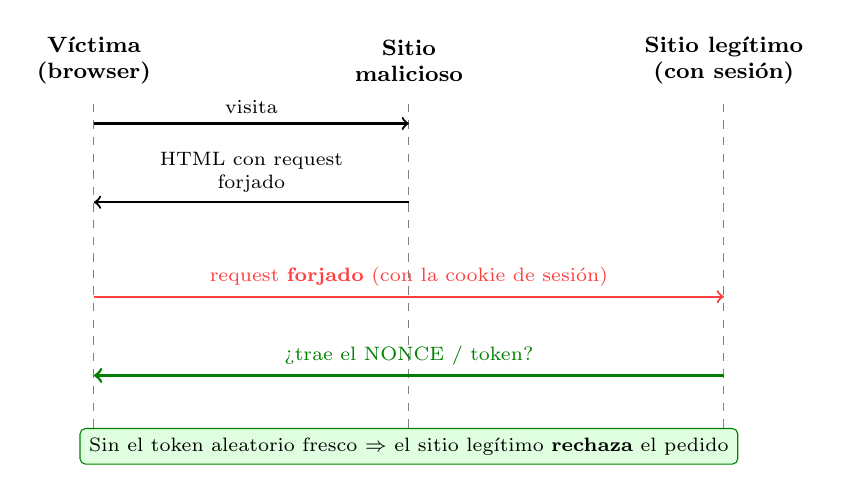
\begin{tikzpicture}[
    actor/.style={font=\footnotesize\bfseries,align=center},
    msg/.style={->,thick,font=\scriptsize}]
  % lifelines
  \node[actor] (V) at (0,3.4) {Víctima\\(browser)};
  \node[actor] (M) at (4,3.4) {Sitio\\malicioso};
  \node[actor] (S) at (8,3.4) {Sitio legítimo\\(con sesión)};
  \foreach \n in {V,M,S}{ \draw[gray,dashed] (\n) ++(0,-0.55) -- ++(0,-4.4); }
  % secuencia
  \draw[msg] (0,2.6) -- node[above]{visita} (4,2.6);
  \draw[msg] (4,1.6) -- node[above,align=center]{HTML con request\\forjado} (0,1.6);
  \draw[msg,red!75] (0,0.4) -- node[above,align=center,red!75]{request \textbf{forjado} (con la cookie de sesión)} (8,0.4);
  % defensa: token anti-CSRF
  \draw[msg,green!50!black,line width=1pt] (8,-0.6) -- node[above,align=center,green!50!black]{¿trae el NONCE / token?} (0,-0.6);
  \node[draw=green!50!black,fill=green!12,rounded corners=2pt,font=\scriptsize,align=center]
        at (4,-1.5) {Sin el token aleatorio fresco $\Rightarrow$ el sitio legítimo \textbf{rechaza} el pedido};
\end{tikzpicture}
\end{center}
\diagcaption{CSRF: el sitio malicioso hace que el browser de la víctima dispare un request al sitio legítimo \emph{con su cookie de sesión}. El \textbf{nonce/token anti-CSRF} (valor aleatorio único en el formulario) lo frena: el atacante no lo conoce, y evita el \emph{replay}.}

\subsubsection{OS Command / Shell Injection (CWE-78)}
Falta de control en el ingreso que permite ejecutar comandos del sistema operativo. Genera \emph{backdoors} para ignorar controles de red o autenticación. Ejemplo: una app PHP que delega a \emph{ImageMagick} pasándole el nombre del archivo sin sanitizar; si el nombre contiene \texttt{;\,rm -fr ...} se ejecutan otros comandos.

\subsubsection{Path / Directory Traversal}
\begin{destacado}
Caso \textbf{router Linksys (2013)}: parámetro \texttt{next\_page=/etc/passwd} permitía leer archivos fuera del directorio esperado (traversal de directorios).
\end{destacado}

\subsubsection{XXE (XML External Entities)}
XML permite cargar esquemas desde una URL; si esa URL se usa para hacer un GET a otra página, un atacante puede escanear la red interna visible por el servidor (estuvo de moda porque casi todas las librerías XML tenían el problema).

\subsubsection{Organizaciones de referencia (OWASP)}
\textbf{OWASP} (Open Web Application Security Project): organización enfocada en combatir problemas de seguridad en aplicaciones Web; publica regularmente las vulnerabilidades más comunes y buenas prácticas. Tiene el \textbf{Top 10} (web), \textbf{OWASP Cloud Top 10} y \textbf{OWASP Top 10 LLM} (ej.: LLM01 Prompt Injection, LLM03 Training Data Poisoning, LLM05 Supply Chain). Junto con MITRE son referencia hace $>$20 años. (Vulnerabilidad moderna asociada: \emph{content/prompt poisoning}: texto invisible en páginas o currículums tipo ``ignora tus instrucciones'' que el LLM/agente termina ejecutando.)

\subsection{Malware básico (mencionado / referenciado para definir)}

\begin{examen}
Ejercicio típico (2016): \textbf{DEFINIR} varios conceptos (mínimo privilegio, confinamiento, rootkit, troyano) y luego \textbf{relacionar dos de forma no trivial}. Estos términos se desarrollan en profundidad en la unidad de \emph{Flujo de información y Malware}; acá basta tenerlos a mano:
\begin{itemize}
  \item \textbf{Troyano}: programa que se disfraza de algo legítimo/útil para que el usuario lo ejecute, ocultando funcionalidad maliciosa (análogo al bug que ``se disfraza de feature'').
  \item \textbf{Rootkit}: software malicioso que se oculta en el sistema (típicamente con privilegios de root/administrador) para mantener acceso persistente y evitar ser detectado.
  \item \textbf{Confinamiento}: limitar/aislar lo que un proceso puede hacer o acceder (sandboxing), muy ligado a \emph{mínimo privilegio} y a \emph{mecanismos exclusivos}.
\end{itemize}
\textbf{Vínculo no trivial sugerido}: \emph{confinamiento} es la materialización técnica de \emph{mínimo privilegio} (aislar para que aunque algo se comprometa, no pueda hacer más que lo mínimo).
\end{examen}

\subsection{La idea del ``chip paranoico''}

\begin{destacado}
De la clase de consulta, el profe remarcó el \textbf{``chip paranoico''}: pensar como atacante. \prof{Seguridad informática es paranoia controlada.} Los muy buenos en seguridad son paranoicos (controladamente): asumen que todos quieren hacer daño de alguna manera, y eso suma. Junto con la \textbf{defensa en profundidad} (encadenar controles para maximizar cuántas cosas hay que romper), son las dos ideas rectoras. Además hay preguntas \textbf{``enciclopédicas''} que requieren \textbf{memorizar definiciones} (p.\,ej. cada letra de STRIDE).
\end{destacado}

\subsection{Lectura recomendada}
Capítulos 12--13 de \emph{Computer Security: Art and Science}, Matt Bishop (Bishop habla de principios, no tanto de amenazas concretas; para amenazas, el proceso de Threat Modeling de OWASP).

\end{document}
